\chapter{Target group analysis}
In this chapter we will investigate the target group of the project. A preliminary assessment will be made to gather information that will help towards the ultimate goal of identifying any special requirements that the target group demands. This will consist of three steps: identifying the target group; describing the target group; and compiling and concluding on the results.

\section{Hj{\o}rring Library: A place for experiences}\label{hjoerring}

%%%% I restructured the whole paragraph, but all the main points are still there. - Marta %%%%
Hj{\o}rring Library aims to distinguish itself from most other Danish libraries. One of the most remarkable things, is the fact that this library is located inside a shopping mall. But once inside, the visitors find themselves into a big open hall with modern architecture. The different sections are divided by bookshelves and a red stripe that goes around the library changing its shape once in a while. The first feeling that the visitors get is that Hj{\o}rring Library is a place where to "hang out" and relax (see figure \ref{fig:p1}, but also have fun or do some work. There are many unique pieces of furniture, creating a great environment for all purposes. Especially kids can have a fun time playing games (physical or digital) and record videos in the children zone (see figures \ref{fig:p2} and \ref{fig:p3}).

At Hj{\o}rring Library the staff has made a big effort on creating an environment as interactive as possible, with many places for people to entertain themselves with other things than just traditional books. Even the cafeteria appears to be part of the library's ordinary environment where people can show up, eat their lunch, drink coffee or just have a beer after work.

\begin{figure}[htbp]\centering
	\begin{minipage}[b]{0.3\textwidth}\centering
		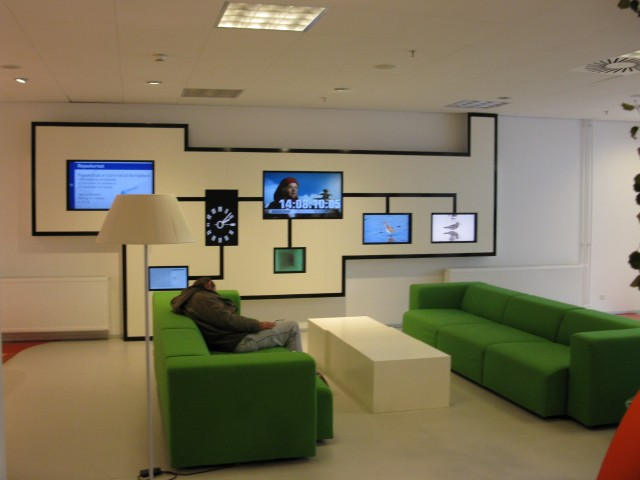
\includegraphics[width=1.00\textwidth]{Pictures/HjoerringLibrary/p1.jpg} %Venstre billede
	\end{minipage}\hfill
	\begin{minipage}[b]{0.3\textwidth}\centering
		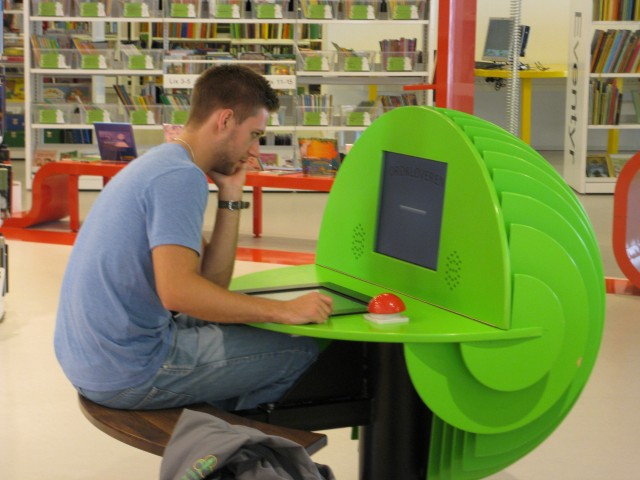
\includegraphics[width=1.00\textwidth]{Pictures/HjoerringLibrary/p2.jpg} %Venstre billede
	\end{minipage}\hfill	
	\begin{minipage}[b]{0.3\textwidth}\centering
		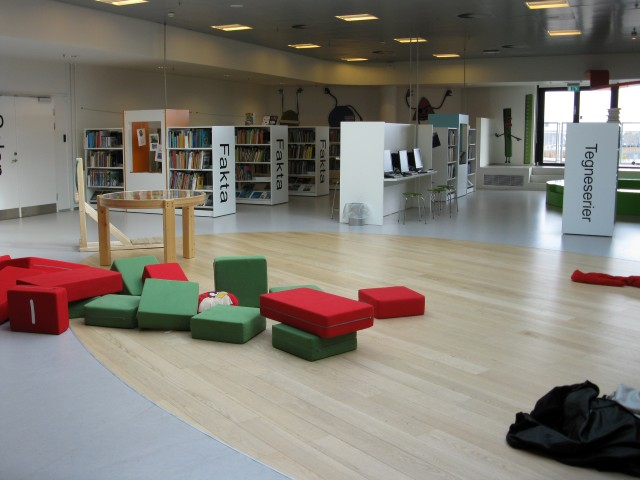
\includegraphics[width=1.00\textwidth]{Pictures/HjoerringLibrary/p3.jpg} %Højre billede
	\end{minipage}\\ %Captions and labels
	\begin{minipage}[t]{0.3\textwidth}
		\caption{Lounge.} %Venstre caption og label
		\label{fig:p1}
	\end{minipage}\hfill
	\begin{minipage}[t]{0.3\textwidth}
		\caption{Playing games.} %Venstre caption og label
		\label{fig:p2}
	\end{minipage}\hfill	
	\begin{minipage}[t]{0.3\textwidth}
		\caption{Physical Angry Birds game} %Højre caption og label
		\label{fig:p3}
	\end{minipage}
\end{figure}

Hj{\o}rring Library gets more than 1000 visitors every day. A way to maintain this number of visitors is by giving them a new and exiting experience every time they come. One way to achieve this is by having various themes that run throughout the whole library, and changing them every six weeks. These includes topics such as: Arabia, birds, fairy tales or simply the color brown. In the period of this project Library Hj{\o}rring has chosen the topic of Christmas, and it will run from the $2^{nd}$ week of November until the last week of December, 2012. By the time the group made the first visit to the library, a bird-theme was running. All kind of birds was exhibited around in the library (see figures \ref{fig:b1} and \ref{fig:b2}), and bird songs were played on the speakers.

\begin{figure}[htbp]\centering
	\begin{minipage}[b]{0.48\textwidth}\centering
		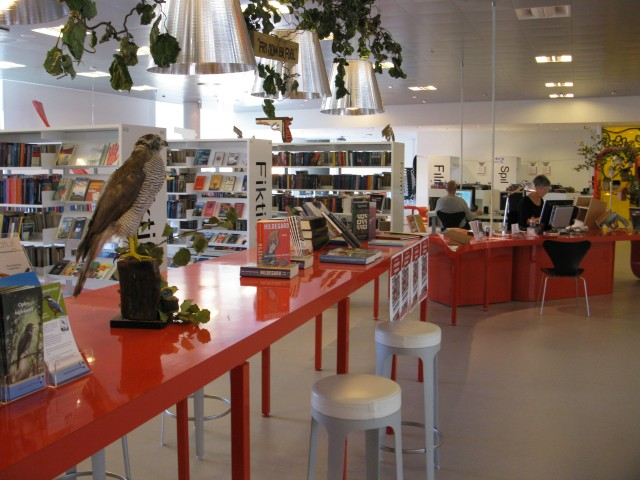
\includegraphics[width=1.00\textwidth]{Pictures/HjoerringLibrary/b1.jpg} %Venstre billede
	\end{minipage}\hfill
	\begin{minipage}[b]{0.48\textwidth}\centering
		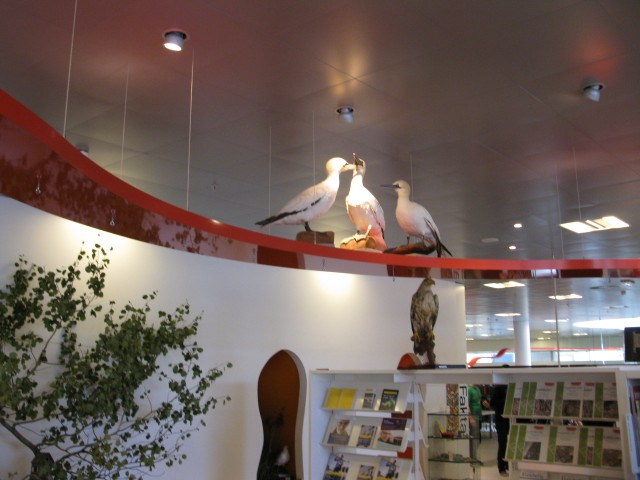
\includegraphics[width=1.00\textwidth]{Pictures/HjoerringLibrary/b2.jpg} %Højre billede
	\end{minipage}\\ %Captions and labels
	\begin{minipage}[t]{0.48\textwidth}
		\caption{Birds.} %Venstre caption og label
		\label{fig:b1}
	\end{minipage}\hfill
	\begin{minipage}[t]{0.48\textwidth}
		\caption{More birds.} %Højre caption og label
		\label{fig:b2}
	\end{minipage}
\end{figure}

These themes are an example of how Hj{\o}rring Library tries to work with the concept of \textit{serendipity}, which basically describes a happy accident; something you didn't expect but turned out to be a pleasant surprise. Even though you go to the library to find a book, you might also experience and learn something that you originally did not expect.

Hj{\o}rring Library is always looking for new projects to involve its visitors in new and engaging ways. As some Medialogy students came previously to do projects, and it turned out to be a success, the staff is eager to try it out again. This is where our group comes into the picture. To us, this is a great opportunity to collaborate with an institution on a project in a "real-life" setting where people outside of the university will interact with the product. Instead of only testing under artificial circumstances, the library will provide us "normal" people to test the project on a day-by-day basis throughout December.

\subsection{Visitor data and placement of the canvas}
The library is divided into several parts, each aiming to give a different experience. As mentioned earlier, it was important for the group to get a central location for the placement of the canvas. This would ensure that a lot of people would have the chance to interact with the program. In fact, the bookshelves finally chosen are just in the middle of the library, so it is almost impossible to not walk past it at some point (see figure \ref{fig:library_floorplans}).

\begin{figure}[htbp]
\centering
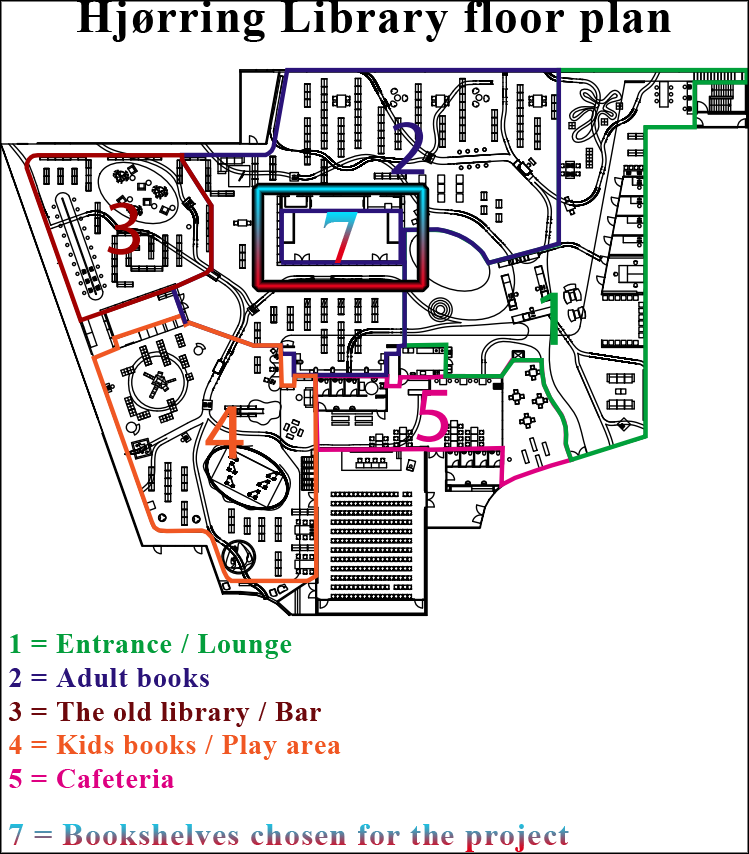
\includegraphics[width=0.80\textwidth]{Pictures/HjoerringLibrary/hjoerring_library_floorplans.png}
\caption{Hj{\o}rring Library is divided into multiple sections. We chose to use a big four-sided bookshelf in the core of the library. Image inspired by \citep{hjoerring_study}.}
\label{fig:library_floorplans}
\end{figure}

%%%%%%%%%%%%%%%%%%%%%%% \citep{hjoerring_study} is shown as [hjo]!!!!!!!!!!!!!!!! %%%%%%%%%%%%%%%%%%%%%%%%

In 2010, \citep{hjoerring_study} did a survey to investigate people's habits and movement pattern at Hj{\o}rring Library. They found that an average visitor spends about half an hour at the library. Those in the age group between 0-10 years and 21-30 years spent most time, 34 and 44 minutes, while those between 41-50 and 61-70 years spent 19 and 26 minutes during a visit.

Several cylinder and flow maps were made to visualize the gathered data. Two are shown in figures \ref{fig:library_cylindermap} and \ref{fig:library_flowmap}.

\begin{figure}[htbp] \centering
\begin{minipage}[b]{0.45\textwidth} \centering
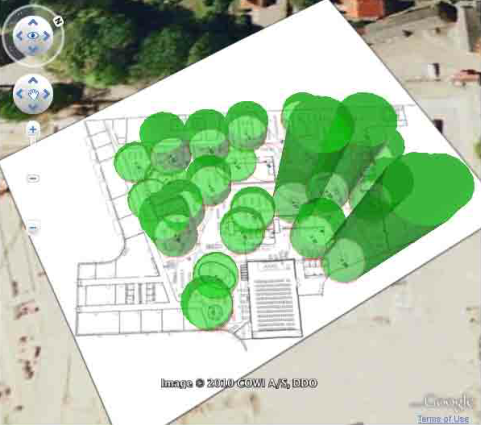
\includegraphics[width=1.00\textwidth]{Pictures/HjoerringLibrary/library_cylinder_diagram_24Nov.png} % Venstre billede
\end{minipage} \hfill
\begin{minipage}[b]{0.45\textwidth} \centering
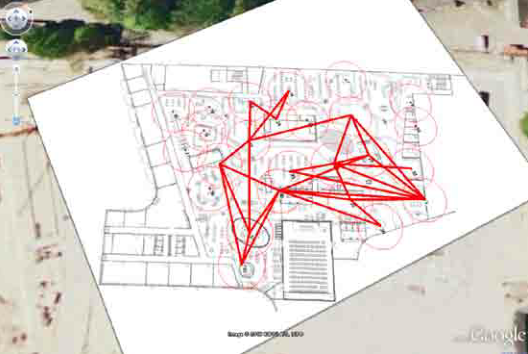
\includegraphics[width=1.00\textwidth]{Pictures/HjoerringLibrary/library_flow_Nov21.png} % Højre billede
\end{minipage} \\ % Captions og labels
\begin{minipage}[t]{0.45\textwidth}
\caption{Cylinder map showing accumulated visiting time at Hj{\o}rring Library Tuesday November 24, 2010. Image created by \citep{hjoerring_study}.} % Venstre caption og label
\label{fig:library_cylindermap}
\end{minipage} \hfill
\begin{minipage}[t]{0.45\textwidth}
\caption{Flow map showing a visitor's movement between 10.20-11.15, Saturday November 21, 2010. Image created by \citep{hjoerring_study}.} % Højre caption og label
\label{fig:library_flowmap}
\end{minipage}
\end{figure}

\section{Identifying the target group}
As the final installation will be available for all visitors at Hj{\o}rring Library, the preliminary identification of the target group should be easily accomplished in this project. Upon visiting the library it becomes apparent that the visitors cover a very large demographic. There are people ranging in age from toddlers, to senior citizens and everything between. To avoid limiting the installation to a specific part of the visitors at the library, the target group was kept as all visitors. And since the program developed during this project is meant as an art installation, and not so much as a practical tool, it seemed unnecessary to try to shoehorn it into a more narrowed target group. That being said, it would be easy to assume that the program would appeal to children, especially when having the Christmas theme in mind. However, there should be no reason for any adult not to try it out.

\section{Description of the target group}
During a small series (sample size was 22 people) of qualitative interviews the group gathered information about the visitors at the library. We were able to gather some information, and use this to create four groups that we will use to categorize the target audience:

\begin{itemize}

\item \textbf{Group 1} \textit{Small children}, the youngest group, were there because their parents enjoyed utilizing the facilities that the library offers. The liked to play around in the kids zone.

\item \textbf{Group 2} \textit{Teens and youngsters} enjoyed spending time at the library while waiting for busses. This gave them the opportunity to enjoy each others company and make use of the computers, games, etc. at the library.

\item \textbf{group 3} \textit{Students} used the library for work, finding literature for reports and writing there. The library have various study rooms that can be used when a quiet place is needed.

\item \textbf{Group 4} Most \textit{adult visitors} used the library to rent material, and not much else. Some people also came to drink coffee at the cafeteria.

\end{itemize}

As well as the interviews, we made several observations during the visit. It is our belief that the teens and youngsters that use the facilities already offered by the library (games, interactive toys, films, etc.) will be the group that would enjoy an additional interactive installation the most.

Generally, the tone at the library is that of any other library, and as such the visitors, mainly students and adult visitors naturally expect a quite and calm working area. This means that the program shouldn't make too much noise, so background music should be kept to a minimum.

\section{Compilation and conclusion}

It is clear that the visitors at the library are a diverse group that all use the library in different ways. When considering an interactive installation in the library, the group that would have the greatest interest in such a thing is the group that also currently use the most of the unique facilities offered by the library: the teens and youngsters. But it is, as mentioned before, important for us to accommodate all groups, so as not to exclude anyone from the audience or end up with too narrow a focus.

It is also a goal for the finished program to fit into the library without disturbing visitors that do not wish to interact with the installation. This means that the final product will not having loud sounds that disturbs visitors.

In order for the installation to be a fun experience for both a casual by-passer, as well as a more interested user, the final program will function on more than one level, this means that you can pass by and admire the installation, but you will also be able to spend more time in front of it, if you want.